\section{Pendahuluan}
\subsection{Latar Belakang}
Seiring berkembangnya zaman—khususnya di sektor teknologi informasi, jaringan komputer menjelma pondasi strategis bagi hampir setiap aspek kehidupan modern: ekonomi digital, e-learning, layanan kesehatan jarak jauh, hingga aktivitas harian seperti menonton YouTube atau melakukan panggilan video. Konektivitas antar-perangkat memfasilitasi pertukaran data yang cepat dan efisien, tetapi sekaligus memunculkan tantangan nyata seperti latensi tinggi, perangkat yang gagal tersambung, manajemen pengguna skala besar, serta ancaman keamanan siber akibat topologi dan konfigurasi yang keliru. \\
Seluruh isu tersebut berpangkal pada kedalaman pemahaman tentang protokol komunikasi, desain topologi, pengalamatan IP, serta penyiapan perangkat keras dan lunak jaringan. Karenanya, praktikum Jaringan Komputer di Laboratorium IoT ini dirancang untuk memberikan pengalaman langsung—mulai dari bagaimana komputer saling terhubung, berkomunikasi, dan bertukar informasi, hingga simulasi kasus yang kerap muncul di lapangan. \\
Modul 1 berperan sebagai landasan: praktikan terlebih dulu menekuni keterampilan crimping kabel UTP agar kabel twisted-pair terpasang sesuai standar T568A demi mengurangi crosstalk, kemudian menyusun skema IPv4 subnetting yang hemat IP address serta menyiapkan routing statis di router inti untuk 4 subnet departemen. 
Dengan rangkaian ini, mahasiswa diharapkan mampu mendiagnosis dan menyelesaikan permasalahan dasar jaringan sekaligus memahami teknologi yang menjadi pondasi internet dan komunikasi digital, sebelum melangkah ke topik lanjutan seperti migrasi IPv6, segmentasi VLAN, dan pelayanan server berbasis cloud.


\section{Dasar Teori}
\subsection{Konsep Jaringan Komputer}
Jaringan komputer adalah ekosistem perangkat keras (end‑device, intermediate device) dan perangkat lunak (protokol) yang memungkinkan pertukaran data terstruktur. IEEE 802 menstandarkan lapisan Data‑Lin untuk berbagai media—Ethernet seperti 802.3, Wi‑Fi, 802.11. Sedangkan IETF bertanggung jawab pada lapisan Internet (IP, ICMP) dan Transport (TCP, UDP).

\subsection{Media Twisted‑Pair dan Crimping}
Kabel UTP (Cat 5e / Cat 6) memiliki impedansi 100Ω dan kecepatan lumayan tinggi, menggunakan differential signaling untuk mereduksi EMI. Dua urutan warna resmi, yakniT568A danT568B yang didesain agar pasangan pins 1↔2 dan 3↔6 tersusun sebagai transmit pair dan receive pair untuk menerima dan mengirim data. Crimping yang benar memastikan insertion loss < 8.0 dB dan return loss >18 dB pada 100MHz (standar ANSITIA‑568.2‑D).

\subsection{Alamat IPv4, CIDR, dan Subnetting}
Alamat IPv4 32‑bit dipecah menjadi bagian network dan host. Metode CIDR (Classless Inter‑Domain Routing) menggantikan pengelompokan kelas klasik dengan notasi a.b.c.d prefix. Rumus kapasitas host valid:
\[N_\text{host}=2^{32-\text{prefix}}-2\]
menyisakan dua alamat khusus (network ID dan broadcast). Pada blok 192.168.1.0/26, tersedia 62 host; sementara blok kecil .../28 hanya memuat 14 host. Subnetting dikombinasikan dengan VLSM untuk meminimalkan ruang kosong.

\subsection{Routing Statis vs Dinamis}
\begin{itemize}
  \item \textbf{Statis}: entri rute dikonfigurasi manual; cocok untuk topologi kecil atau \emph{edge network}. Tidak menambah overhead CPU maupun bandwidth, tetapi rawan human error saat topologi berubah.
  \item \textbf{Dinamis}: router saling bertukar informasi menggunakan protokol—RIP (v2), OSPF (v2 dan 3), EIGRP. Fiturauto‑reconvergence meningkatkan ketersediaan, namun membutuhkan sumber daya.
\end{itemize}

\subsection{Pemantauan Jaringan dengan Wireshark}
Wireshark menangkap paket menggunakan pustaka libpcap / WinPcap. Filter BPF (e.g., ip.addr==192.168.1.1) menyaring data agar analisis lebih fokus. Fitur expert info secara otomatis menandai anomali—duplicate ACK, TCPretransmission—mempercepat diagnosa.

\subsection{File \texttt{.pcap} dan Replikas Uji}
File \texttt{.pcap} menyimpan frame secara berurutan disertai stempel waktu epoch. Hal ini memungkinkan praktikan melakukan offline replay menggunakan tcpreplay untuk menguji firewall tanpa mengganggu trafik produksi.

\subsection{Siklus Troubleshooting OSI}
Metode “\emph{bottom‑up}” dimulai dengan continuity test kabel (Layer 1), verifikasi link LED (Layer 2), pengecekan IP address (Layer 3), ping dan traceroute (Layer 3 dan 4), hingga penelusuran sesi HTTP dengan developer tools (Layer 7). Prinsip ini melatih praktikan berpikir sistematis.

%===========================================================%
\section{Tugas Pendahuluan}
Bagian ini berisi jawaban dari tugas pendahuluan yang telah anda kerjakan, beserta penjelasan dari jawaban tersebut
\begin{enumerate}
	\item \textbf{Perencanaan Subnet}\newline
        Tabel \ref{tab:cidr} menunjukkan pemilihan prefix agar alamat tidak terbuang.
        \begin{table}[H]
        \centering
        \caption{Penentuan prefix CIDR}
        \label{tab:cidr}
        \begin{tabular}{|l|c|c|c|}
          \hline
          Departemen & Jumlah Perangkat & Prefix & \# IP Tersedia \\
          \hline
          Produksi & 50 & /26 & 64 \\
          Administrasi & 20 & /27 & 32 \\
          Keuangan & 10 & /28 & 16 \\
          R\&D & 100 & /25 & 128 \\
          \hline
        \end{tabular}
        \end{table}
        Dengan blok privat \texttt{192.168.1.0\/24} dibagi sebagai berikut:
        
        \begin{table}[H]
        \centering
        \begin{tabular}{|l|c|c|c|c|}
          \hline
          Departemen & Subnet & Rentang Host & Broadcast & Gateway \\
          \hline
          Produksi & 192.168.1.0/26 & 192.168.1.1 – 192.168.1.62 & 192.168.1.63 & 192.168.1.1 \\
          Administrasi & 192.168.1.64/27 & 192.168.1.65 – 192.168.1.94 & 192.168.1.95 & 192.168.1.65 \\
          Keuangan & 192.168.1.96/28 & 192.168.1.97 – 192.168.1.110 & 192.168.1.111 & 192.168.1.97 \\
          R\&D & 192.168.1.112/25 & 192.168.1.113 – 192.168.1.254 & 192.168.1.255 & 192.168.1.113 \\
          \hline
        \end{tabular}
        \end{table}

    \item \textbf{Diagram Topologi}\newline
        \begin{figure}[H]
          \centering
          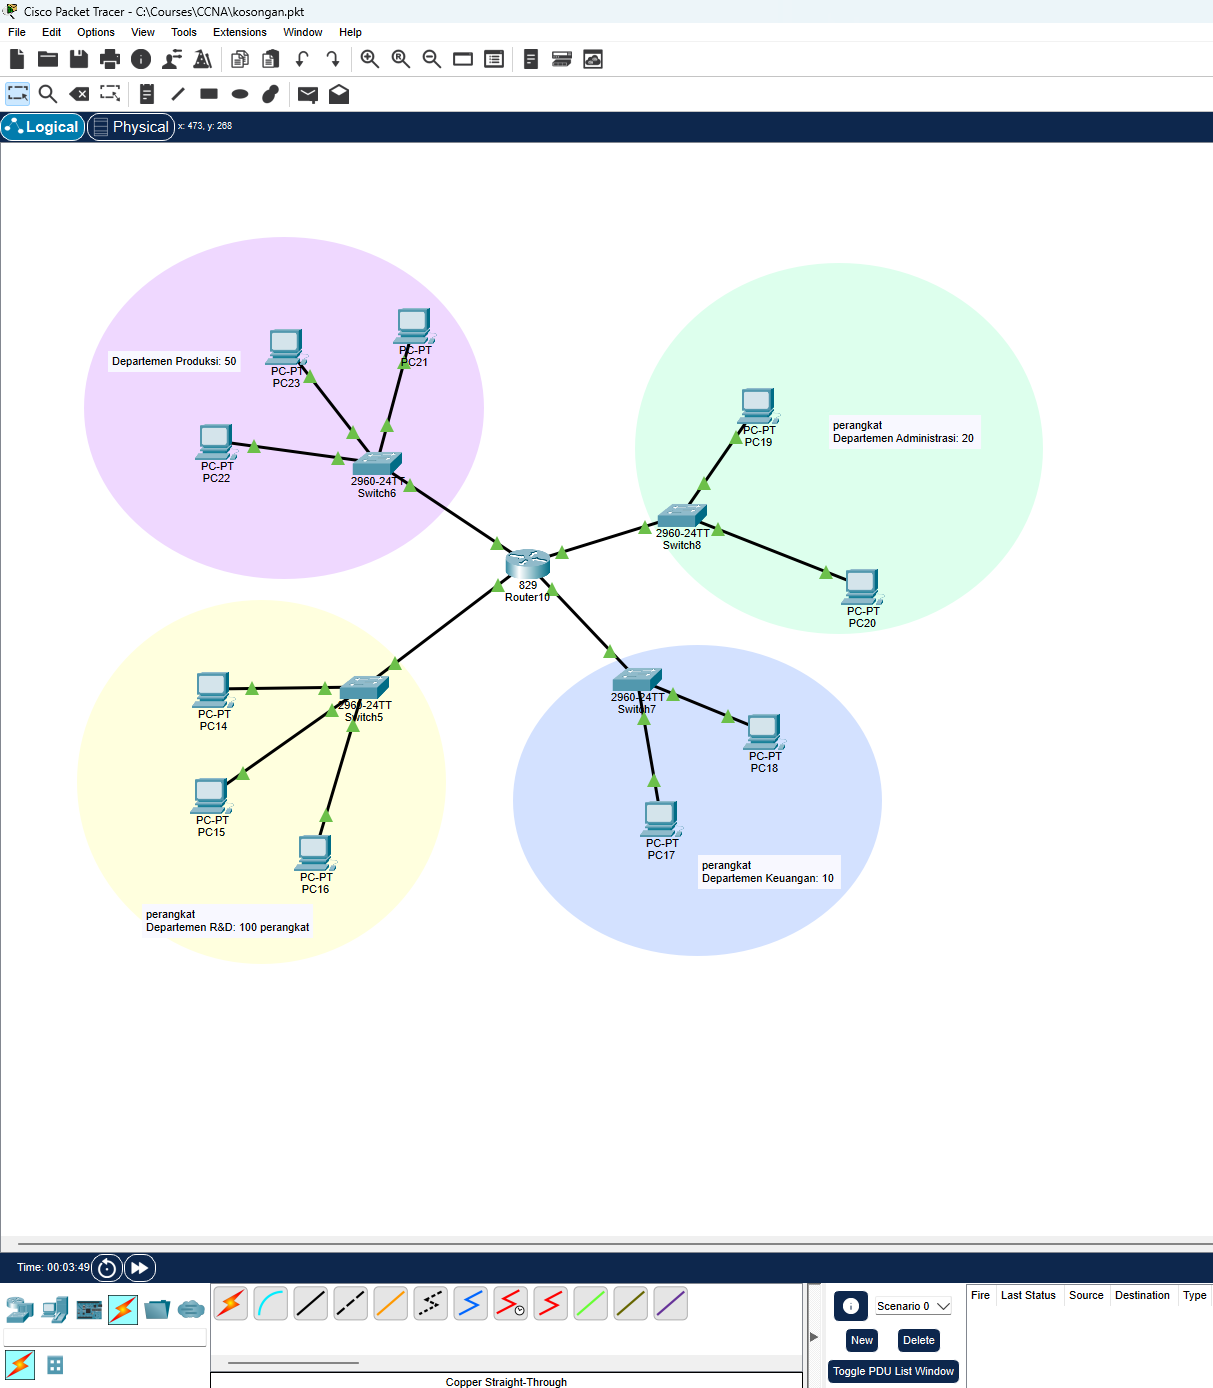
\includegraphics[width=\linewidth,height=12cm,keepaspectratio]{P1/img/Topologi.png}
          \caption{topologi jaringan untuk small enterprise antar departemen}
          \label{fig:topologi}
        \end{figure}
        % Ganti framebox di atas dengan \includegraphics{img/topologi_small_enterprise.pdf}
    
	\item \textbf{Tabel Routing Router Utama}\newline
        \begin{table}[H]
        \centering
        \begin{tabular}{|l|c|c|c|}
          \hline
          Network Destination & Netmask\/Prefix & Gateway & Interface \\
          \hline
          192.168.1.0 & 255.255.255.192 (/26) & -- & eth0 \\
          192.168.1.64 & 255.255.255.224 (/27) & -- & eth2 \\
          192.168.1.96 & 255.255.255.240 (/28) & -- & eth1 \\
          192.168.1.112 & 255.255.255.128 (/25) & -- & eth3 \\
          0.0.0.0 & 0.0.0.0 (/0) & ISP Gateway & WAN \\
          \hline
        \end{tabular}
        \caption{Routing table router utama}
        \end{table}
        
	\item \textbf{Pemilihan Metode Routing}\newline
        Berdasarkan kompleksitas topologi dan keterbatasan sumber daya, static routing dipilih dengan pertimbangan:
        \begin{enumerate}[label=\alph*)]
          \item \textbf{Sederhana dan deterministik} — hanya terdapat satu router inti yang meneruskan paket ke empat subnet internal sehingga jalur tidak berubah‑ubah.
          \item \textbf{Skala jaringan kecil} — total 180 host masih di bawah ambang batas praktik statik ( \textless500 host).
          \item \textbf{Hemat CPU \& bandwidth} — router SOHO kelas entry tidak perlu memproses paket hello \& update, menghemat ±3–5 \% utilisasi CPU serta ±32 kbps konsumsi link.
          \item \textbf{Kemudahan troubleshooting} — tabel rute dapat diaudit manual; kesalahan konfigurasi (misal typo subnet) langsung terdeteksi tanpa menunggu convergence protokol dinamis.
        \end{enumerate}
        \vspace{3pt}
        \noindent\textbf{Rencana Skalabilitas}\newline
        Jika jumlah subnet meningkat atau dibutuhkan redundansi jalur, administrator dapat bermigrasi ke protokol dinamis yang sesuai:
        \begin{itemize}
          \item \textbf{RIP v2} — simpel, mendukung VLSM, cocok untuk flat network hingga 15hop.
          \item \textbf{OSPF}— berbasis link‑state, konvergen cepat, ideal untuk topologi mesh antar kantor.
        \end{itemize}

\end{enumerate}